\documentclass[12 pt]{article}

\usepackage{amsfonts, amssymb, amsmath}
\usepackage{graphicx}
\usepackage{subcaption} 
\usepackage{float}
\usepackage{listings}

\usepackage{xcolor}

\definecolor{codegreen}{rgb}{0,0.6,0}
\definecolor{codegray}{rgb}{0.5,0.5,0.5}
\definecolor{codepurple}{rgb}{0.58,0,0.82}
\definecolor{backcolour}{rgb}{0.95,0.95,0.92}

\lstdefinestyle{mystyle}{
    backgroundcolor=\color{backcolour},   
    commentstyle=\color{codegreen},
    keywordstyle=\color{magenta},
    numberstyle=\tiny\color{codegray},
    stringstyle=\color{codepurple},
    basicstyle=\ttfamily\footnotesize,
    breakatwhitespace=false,         
    breaklines=true,                 
    captionpos=b,                    
    keepspaces=true,                 
    numbers=left,                    
    numbersep=5pt,                  
    showspaces=false,                
    showstringspaces=false,
    showtabs=false,                  
    tabsize=2
}

\lstset{style=mystyle}

\oddsidemargin=-0.5cm
\setlength{\textwidth}{6.5in}
\addtolength{\voffset}{-20pt}
\addtolength{\headsep}{25pt}

\pagestyle{myheadings}

\markright{
    \begin{minipage}[t]{0.5\textwidth}
        Joseph González Pastora \\
        Gabriel Gutierrez Arguedas \\
        Ricardo Sánchez Alpízar
    \end{minipage}
    \hfill
    \begin{minipage}[t]{0.3\textwidth}
        \centering
        Septiembre 1, 2024
    \end{minipage}
}

\newcommand{\eqn}[0]{\begin{array}{rcl}}
\newcommand{\eqnend}[0]{\end{array} }
\newcommand{\qed}[0]{$\square$}

\begin{document}

\section{Sistemas Lineales (40 puntos)}

\begin{enumerate}
    
\item Demuestre si los siguientes sistemas ${L\{ \cdot \}}$ (con entrada ${u(t)}$ y salida ${g(t)}$, y ${h(t)}$ una función cualquiera) son lineales o no lineales. Además, muestrelo con una implementación en Pytorch, usando como entrada un arreglo de 50 valores generados al azar. Si va a demostrar por contraejemplo, muestre las entradas y salidas de la corrida en Pytorch que demuestran el no cumplimiento de la propiedad.

\begin{enumerate}
    \item ${g(t)=u(t)+3}$
    \item ${g(t)=u(t)h(t)}$ 
    \item ${g(t)=max(u(t))}$
    \item ${g(t)=|u(t)|}$
\end{enumerate}

\subsection{Respuesta 1.1.a}
\label{1pA}

Aplicando el operador ${L\{ \cdot \}}$ a el sistema ${g(t)=u(t)+3}$, y utilizando una entrada dada por ${u(t)=\alpha u_{1}(t) + \beta u_{2}(t)}$ se tiene:

\begin{equation}
\label{sist1a1}
    L\{ \alpha u_{1}(t) + \beta u_{2}(t) \} = \alpha u_{1}(t) + \beta u_{2}(t) + 3 
\end{equation}

Para que un sistema sea lineal debe cumplir la propiedad de superposición y homogeneidad. Aplicados al sistema se tiene:

\begin{center}
\begin{equation} \label{sist1a2}
\begin{split}
 L\{ \alpha u_{1}(t) + \beta u_{2}(t) \} = \alpha L\{ u_{1}(t) \} + \beta L\{ u_{2}(t) \} \\
 = \alpha (u_{1}(t)+3) + \beta (u_{2}(t)+3) = \alpha u_{1}(t) + \beta u_{2}(t) + 6
\end{split}
\end{equation}
\end{center}

Como el resultado de la ecuación (\ref{sist1a1}) es distinta al de la ecuación (\ref{sist1a2}), se puede concluir que el sistema no es lineal.

Para corroborar el resultado usando PyTorch se crean las entradas ${u_{1}(t)}$ y ${u_{2}(t)}$ y se establecen lo valores de ${\alpha}$ y ${\beta}$ de forma aleatoria:

\begin{lstlisting}[language=Python]
u1 = torch.rand(50)
u2 = torch.rand(50) 
alpha = torch.rand(1)
beta = torch.rand(1)

print(f"Entrada u1(t): \n{u1}")
print(f"Entrada u2(t): \n{u2}")
print(f"alpha: {alpha}")
print(f"beta: {beta}")
\end{lstlisting}

Obteniendo: 

\begin{lstlisting}
Entrada u1(t): 
tensor([0.3948, 0.6505, 0.5344, 0.2316, 0.8186, 0.8870, 0.5365, 0.9284, 0.2808,
        0.2539, 0.1339, 0.2282, 0.1158, 0.4595, 0.1076, 0.2796, 0.0177, 0.3978,
        0.0852, 0.0741, 0.6352, 0.3848, 0.5970, 0.1469, 0.3017, 0.0665, 0.0943,
        0.4978, 0.2756, 0.3077, 0.8043, 0.3984, 0.9700, 0.1766, 0.2735, 0.2933,
        0.5566, 0.5119, 0.2545, 0.7325, 0.3498, 0.0764, 0.4299, 0.0310, 0.8868,
        0.1638, 0.0759, 0.3081, 0.5356, 0.6004])
Entrada u2(t): 
tensor([0.0293, 0.8738, 0.2842, 0.7869, 0.7953, 0.9265, 0.6366, 0.6660, 0.9436,
        0.4315, 0.4577, 0.0614, 0.8657, 0.5970, 0.0833, 0.6582, 0.9319, 0.9057,
        0.7067, 0.3079, 0.3431, 0.9982, 0.5889, 0.8578, 0.9616, 0.0214, 0.4284,
        0.2320, 0.6360, 0.4911, 0.5137, 0.8629, 0.8284, 0.1537, 0.5002, 0.7349,
        0.3355, 0.2836, 0.3027, 0.7798, 0.3587, 0.7845, 0.7481, 0.4064, 0.3958,
        0.5576, 0.9659, 0.8698, 0.1593, 0.6550])
alpha: tensor([0.1505])
beta: tensor([0.2789])
\end{lstlisting}

Para que un sistema sea lineal el resultado de aplicar el operador ${L\{ \cdot \}}$ con la entrada escogida debe ser igual al de aplicar la superposición y la homogeneidad. Se utiliza la función equal() de PyTorch para comparar si los resultados son iguales:

\hspace{1mm}

\begin{lstlisting}[language=Python]
def compare_outputs(u, v):
    if torch.equal(u, v):
        print("Las salidas son iguales, se cumple la superposicion y la homogeneidad")
    else:
        print("Las salidas no son iguales, no se cumple la superposicion y la homogeneidad")
\end{lstlisting}

Computando las ecuaciones (\ref{sist1a1}) y (\ref{sist1a2}):

\begin{lstlisting}[language=Python]
L_input = alpha*u1 + (beta*u2) + 3
print(f"alpha*u1 + beta*u2 + 3: \n{L_input}\n")

L_linear = alpha*u1 + beta*u2 + 6
print(f"alpha*u1 + beta*u2 + 6: \n{L_linear}\n")

compare_outputs(L_input, L_linear)
\end{lstlisting}

Se obtiene:

\begin{lstlisting}
alpha*u1 + beta*u2 + 3: 
tensor([3.0676, 3.3416, 3.1597, 3.2543, 3.3450, 3.3919, 3.2583, 3.3255, 3.3054,
        3.1585, 3.1478, 3.0515, 3.2588, 3.2356, 3.0394, 3.2256, 3.2625, 3.3124,
        3.2099, 3.0970, 3.1913, 3.3363, 3.2541, 3.2613, 3.3136, 3.0160, 3.1336,
        3.1396, 3.2189, 3.1833, 3.2643, 3.3006, 3.3770, 3.0694, 3.1807, 3.2491,
        3.1773, 3.1561, 3.1227, 3.3277, 3.1527, 3.2303, 3.2733, 3.1180, 3.2439,
        3.1801, 3.2808, 3.2889, 3.1250, 3.2730])

alpha*u1 + beta*u2 + 6: 
tensor([6.0676, 6.3416, 6.1597, 6.2543, 6.3450, 6.3919, 6.2583, 6.3255, 6.3054,
        6.1585, 6.1478, 6.0515, 6.2588, 6.2356, 6.0394, 6.2256, 6.2625, 6.3124,
        6.2099, 6.0970, 6.1913, 6.3363, 6.2541, 6.2613, 6.3136, 6.0160, 6.1336,
        6.1396, 6.2189, 6.1833, 6.2643, 6.3006, 6.3770, 6.0694, 6.1807, 6.2491,
        6.1773, 6.1561, 6.1227, 6.3277, 6.1527, 6.2303, 6.2733, 6.1180, 6.2439,
        6.1801, 6.2808, 6.2889, 6.1250, 6.2730])

Las salidas no son iguales, no se cumple la superposicion y la homogeneidad
\end{lstlisting}

Con resultados distintos, se demuestra la no linealidad del sistema.

\subsection{Respuesta 1.1.b}

Aplicando el operador ${L\{ \cdot \}}$ a el sistema ${g(t)=u(t)h(t)}$, y utilizando una entrada dada por ${u(t)=\alpha u_{1}(t) + \beta u_{2}(t)}$ se tiene:

\begin{equation}
\label{sist2a1}
    L\{ \alpha u_{1}(t) + \beta u_{2}(t) \} = \alpha u_{1}(t)h(t) + \beta u_{2}(t)h(t) 
\end{equation}

Para que un sistema sea lineal debe cumplir la propiedad de superposición y homogeneidad. Aplicados al sistema se tiene:

\begin{center}
\begin{equation} \label{sist2a2}
\begin{split}
 L\{ \alpha u_{1}(t) + \beta u_{2}(t) \} = \alpha L\{ u_{1}(t) \} + \beta L\{ u_{2}(t) \} \\
 = \alpha u_{1}(t)h(t) + \beta u_{2}(t)u(t)
\end{split}
\end{equation}
\end{center}

Como el resultado de la ecuación (\ref{sist2a1}) es igual al de la ecuación (\ref{sist2a2}), se puede concluir que el sistema es lineal. Es importante aclarar que esta linealidad se mantiene sí y sólo sí ${h(t)}$ es totalmente independiente de ${u(t)}$.

Para corroborar el resultado usando PyTorch se utilizan las mismas entradas generadas de forma aleatoria y la función para comparar los resultados mostradas en la sección \ref{1pA}.

Computando las ecuaciones (\ref{sist2a1}) y (\ref{sist2a2}):

\begin{lstlisting}[language=Python]
# Creando una funcion h cualquiera
h = torch.rand(50)

L_input = (alpha*u1*h) + (beta*u2*h)
print(f"alpha*u*h + beta*u*h: \n{L_input}\n")

L_linear = (alpha*u1*h) + (beta*u2*h)
print(f"(alpha*u*h) + (beta*u*h): \n{L_linear}\n")

compare_outputs(L_input, L_linear)
\end{lstlisting}

Se obtiene:

\begin{lstlisting}
(alpha*u*h) + (beta*u*h): 
tensor([0.0525, 0.2011, 0.1107, 0.1648, 0.1427, 0.1827, 0.1227, 0.0839, 0.0460,
        0.0735, 0.0450, 0.0153, 0.2213, 0.2005, 0.0188, 0.0730, 0.0869, 0.2727,
        0.0952, 0.0181, 0.1328, 0.0252, 0.1397, 0.0492, 0.1351, 0.0056, 0.0412,
        0.1358, 0.0886, 0.0880, 0.1904, 0.0501, 0.2692, 0.0420, 0.1378, 0.2099,
        0.1128, 0.1374, 0.0167, 0.0367, 0.1010, 0.1794, 0.0064, 0.1154, 0.1640,
        0.0892, 0.1707, 0.2625, 0.0582, 0.0227])

(alpha*u*h) + (beta*u*h): 
tensor([0.0525, 0.2011, 0.1107, 0.1648, 0.1427, 0.1827, 0.1227, 0.0839, 0.0460,
        0.0735, 0.0450, 0.0153, 0.2213, 0.2005, 0.0188, 0.0730, 0.0869, 0.2727,
        0.0952, 0.0181, 0.1328, 0.0252, 0.1397, 0.0492, 0.1351, 0.0056, 0.0412,
        0.1358, 0.0886, 0.0880, 0.1904, 0.0501, 0.2692, 0.0420, 0.1378, 0.2099,
        0.1128, 0.1374, 0.0167, 0.0367, 0.1010, 0.1794, 0.0064, 0.1154, 0.1640,
        0.0892, 0.1707, 0.2625, 0.0582, 0.0227])

Las salidas son iguales, se cumple la superposicion y la homogeneidad
\end{lstlisting}

Con resultados iguales, se demuestra la linealidad del sistema.

\subsection{Respuesta 1.1.c}

Aplicando el operador ${L\{ \cdot \}}$ a el sistema ${g(t)=max(u(t))}$, y utilizando una entrada dada por ${u(t)=\alpha u_{1}(t) + \beta u_{2}(t)}$ se tiene:

\begin{equation}
\label{sist3a1}
    L\{ \alpha u_{1}(t) + \beta u_{2}(t) \} = max(\alpha u_{1}(t) + \beta u_{2}(t)) 
\end{equation}

Para que un sistema sea lineal debe cumplir la propiedad de superposición y homogeneidad. Aplicados al sistema se tiene:

\begin{center}
\begin{equation} \label{sist3a2}
\begin{split}
 L\{ \alpha u_{1}(t) + \beta u_{2}(t) \} = \alpha L\{ u_{1}(t) \} + \beta L\{ u_{2}(t) \} \\
 = \alpha max(u_{1}(t)) + \beta max(u_{2}(t))
\end{split}
\end{equation}
\end{center}

Como el resultado de la ecuación (\ref{sist3a1}) es distinta al de la ecuación (\ref{sist3a2}), se puede concluir que el sistema no es lineal.

Para corroborar el resultado usando PyTorch se utilizan las mismas entradas generadas de forma aleatoria y la función para comparar los resultados mostradas en la sección \ref{1pA}.

Computando las ecuaciones (\ref{sist3a1}) y (\ref{sist3a2}):

\begin{lstlisting}[language=Python]{myc,label=compare}
L_input = torch.max(alpha*u1 + beta*u2)
print(f"max(alpha*u1 + beta*u2): \n{L_input}\n")

L_linear = alpha*torch.max(u1) + beta*torch.max(u2)
print(f"alpha*torch.max(u1) + beta*torch.max(u2): \n{L_linear}\n")

compare_outputs(L_input, L_linear)
\end{lstlisting}

Se obtiene:

\begin{lstlisting}
max(alpha*u1 + beta*u2): 
0.3918687105178833

alpha*torch.max(u1) + beta*torch.max(u2): 
tensor([0.4244])

Las salidas no son iguales, no se cumple la superposicion y la homogeneidad
\end{lstlisting}

Con resultados distintos, se demuestra la no linealidad del sistema.

\subsection{Respuesta 1.1.d}

Aplicando el operador ${L\{ \cdot \}}$ a el sistema ${g(t)=|u(t)|}$, y utilizando una entrada dada por ${u(t)=\alpha u_{1}(t) + \beta u_{2}(t)}$ se tiene:

\begin{equation}
\label{sist4a1}
    L\{ \alpha u_{1}(t) + \beta u_{2}(t) \} = |\alpha u_{1}(t) + \beta u_{2}(t)| 
\end{equation}

Para que un sistema sea lineal debe cumplir la propiedad de superposición y homogeneidad. Aplicados al sistema se tiene:

\begin{center}
\begin{equation} \label{sist4a2}
\begin{split}
 L\{ \alpha u_{1}(t) + \beta u_{2}(t) \} = \alpha L\{ u_{1}(t) \} + \beta L\{ u_{2}(t) \} \\
 = \alpha |u_{1}(t)| + \beta |u_{2}(t)|
\end{split}
\end{equation}
\end{center}

Como el resultado de la ecuación (\ref{sist4a1}) es equivalente al de la ecuación (\ref{sist4a2}) sí y sólo sí ${\alpha \geq 0}$ y ${\beta \geq 0}$ y el sistema es lineal. Para ${\alpha}$ y ${\beta}$ negativos el sistema es no lineal.

Para corroborar el resultado usando PyTorch se utilizan las mismas entradas generadas de forma aleatoria y la función para comparar los resultados mostradas en la sección \ref{1pA}.

Computando las ecuaciones (\ref{sist4a1}) y (\ref{sist4a2}):

\begin{lstlisting}[language=Python]{myc,label=compare}
L_input = torch.abs(alpha*u1 + beta*u2)
print(f"|alpha*u1 + beta*u2|: \n{L_input}\n")

L_linear = alpha*torch.abs(u1) + beta*torch.abs(u2)
print(f"alpha*torch.abs(u1) + beta*torch.abs(u2): \n{L_linear}\n")

compare_outputs(L_input, L_linear)
\end{lstlisting}

Obteniendo:

\begin{lstlisting}
|alpha*u1 + beta*u2|: 
tensor([0.0676, 0.3416, 0.1597, 0.2543, 0.3450, 0.3919, 0.2583, 0.3255, 0.3054,
        0.1585, 0.1478, 0.0515, 0.2588, 0.2356, 0.0394, 0.2256, 0.2625, 0.3124,
        0.2099, 0.0970, 0.1913, 0.3363, 0.2541, 0.2613, 0.3136, 0.0160, 0.1336,
        0.1396, 0.2189, 0.1833, 0.2643, 0.3006, 0.3770, 0.0694, 0.1807, 0.2491,
        0.1773, 0.1561, 0.1227, 0.3277, 0.1527, 0.2303, 0.2733, 0.1180, 0.2439,
        0.1801, 0.2808, 0.2889, 0.1250, 0.2730])

alpha*torch.abs(u1) + beta*torch.abs(u2): 
tensor([0.0676, 0.3416, 0.1597, 0.2543, 0.3450, 0.3919, 0.2583, 0.3255, 0.3054,
        0.1585, 0.1478, 0.0515, 0.2588, 0.2356, 0.0394, 0.2256, 0.2625, 0.3124,
        0.2099, 0.0970, 0.1913, 0.3363, 0.2541, 0.2613, 0.3136, 0.0160, 0.1336,
        0.1396, 0.2189, 0.1833, 0.2643, 0.3006, 0.3770, 0.0694, 0.1807, 0.2491,
        0.1773, 0.1561, 0.1227, 0.3277, 0.1527, 0.2303, 0.2733, 0.1180, 0.2439,
        0.1801, 0.2808, 0.2889, 0.1250, 0.2730])

Las salidas son iguales, se cumple la superposicion y la homogeneidad
\end{lstlisting}

Los valores de ${\alpha}$ y ${\beta}$ son mayores a 0, por lo que se demuestra la linealidad para este caso.

\item Demuestre si los siguientes sistemas con múltiples variables
de entrada ${L\{ \cdot \}}$ (con entrada vectorial ${\vec{u}}$ y salida escalar ${s}$ ${\epsilon}$ ${\mathbb{R}}$), cumplen la condición de homogeneidad absoluta (${L\{ rx \} = |r|L\{ x \}}$) y superposición. Además, muestrelo con una implementación en Pytorch, mostrando la propiedad con 50 vectores generados al azar. Si realiza la demostración por contraejemplo, muestre las entradas y salidas de la corrida en PyTorch que demuestran el no cumplimiento de la propiedad.

\begin{enumerate}
    \item Norma de Manhattan ${\ell_{1}}$
    \item Norma Euclidiana ${\ell_{2}}$
    \item Norma ${\ell_{\infty}}$
\end{enumerate}

\subsection{Respuesta 1.2.a}

Aplicando el operador ${L\{ \cdot \}}$ a la norma ${\ell_{1}}$, y utilizando una entrada dada por ${\vec{u}=\alpha \vec{u_{1}} + \beta \vec{u_{2}}}$ se tiene:

\begin{center}
\begin{equation} \label{l11}
\begin{split}
 ||\vec{u}||_{1} = \sum_{i=1}^{n} |u_{i}| = \sum_{i=1}^{n} |\alpha u_{1i} + \beta u_{2i}| \\
 = |\alpha u_{11} + \beta u_{21}| + |\alpha u_{12} + \beta u_{22}| + \cdots + |\alpha u_{1n} + \beta u_{2n}|
\end{split}
\end{equation}
\end{center}

Para que un sistema sea lineal debe cumplir la propiedad de superposición y homogeneidad. Aplicados a la norma ${\ell_{1}}$ se tiene:

\begin{center}
\begin{equation} \label{l12}
\begin{split}
 ||\vec{u}||_{1} = \sum_{i=1}^{n} |u_{i}| = \sum_{i=1}^{n} |\alpha u_{1i}| + \sum_{i=1}^{n} |\beta u_{2i}| \\
 = |\alpha| (|u_{11}| + |u_{12}| + \cdots + |u_{1n}|) + |\beta| (|u_{21}| + |u_{22}| + \cdots + |u_{2n}|)
\end{split}
\end{equation}
\end{center}

Como el resultado de la ecuación (\ref{l11}) es distinta al de la ecuación (\ref{l12}), se puede concluir que el sistema no es lineal. Un contra ejemplo que también lo demuestra es cuando ${|\alpha u_{1i}}$ y ${u_{2i}|}$ tienen signos opuestos

Para corroborar el resultado usando PyTorch se crean de forma aleatoria las entradas ${u_{1}(t)}$ y ${u_{2}(t)}$ como matrices 50x5 y se trabaja cada fila como un vector individual 1x5. Los valores de ${\alpha}$ y ${\beta}$ de también son aleatorios:

\begin{lstlisting}[language=Python]
u1 = torch.rand(50, 5)
u2 = torch.rand(50, 5)
alpha = torch.rand(1)
beta = torch.rand(1)

print(f"Entradas u1(t): \n{u1}")
print(f"Entradas u2(t): \n{u2}")
print(f"alpha: {alpha}")
print(f"beta: {beta}")
\end{lstlisting}

Obteniendo:

\begin{lstlisting}
Entradas u1(t): 
tensor([[0.1751, 0.7456, 0.0430, 0.3133, 0.8769],
        [0.1766, 0.4136, 0.4713, 0.5058, 0.0309],
        [0.4540, 0.7546, 0.2295, 0.8348, 0.6230],
        [0.7478, 0.2239, 0.7385, 0.8737, 0.1183],
        [0.6758, 0.5630, 0.2625, 0.6088, 0.3537],
        [0.8431, 0.2797, 0.5115, 0.1808, 0.4336],
        [0.1587, 0.0877, 0.9632, 0.7523, 0.2306],
        [0.2057, 0.3903, 0.6914, 0.6748, 0.3663],
        [0.8800, 0.5820, 0.5934, 0.4510, 0.7466],
        [0.1817, 0.9595, 0.9380, 0.8771, 0.0033],
        [0.3493, 0.9485, 0.3859, 0.3669, 0.5327],
        [0.4426, 0.0879, 0.5392, 0.8971, 0.3727],
        [0.2036, 0.3325, 0.6793, 0.5595, 0.1617],
        [0.5445, 0.7438, 0.9290, 0.4616, 0.8586],
        [0.9580, 0.9850, 0.9010, 0.7862, 0.4043],
        [0.4098, 0.3256, 0.4196, 0.1446, 0.2404],
        [0.2521, 0.6592, 0.7047, 0.9881, 0.8459],
        [0.9812, 0.0566, 0.9014, 0.6449, 0.7836],
        [0.5029, 0.9217, 0.4498, 0.4050, 0.5619],
        [0.7552, 0.4734, 0.6934, 0.3650, 0.4470],
        [0.8465, 0.7620, 0.7126, 0.0720, 0.0438],
        [0.7713, 0.0950, 0.2657, 0.6715, 0.9205],
        [0.2648, 0.6370, 0.8133, 0.7911, 0.3547],
        [0.4821, 0.9361, 0.5279, 0.7838, 0.0690],
        [0.4049, 0.7357, 0.9831, 0.5369, 0.9055],
        [0.8316, 0.8629, 0.2338, 0.3087, 0.2101],
        [0.8486, 0.0363, 0.1356, 0.5643, 0.0955],
        [0.0605, 0.6609, 0.5182, 0.3907, 0.3697],
        [0.4237, 0.7653, 0.8285, 0.2559, 0.9851],
        [0.7601, 0.8760, 0.9435, 0.0587, 0.5315],
        [0.8872, 0.5916, 0.7647, 0.9836, 0.4009],
        [0.8086, 0.6844, 0.4439, 0.7758, 0.1151],
        [0.4432, 0.1335, 0.0720, 0.8316, 0.1769],
        [0.4199, 0.3766, 0.0841, 0.4100, 0.1196],
        [0.0778, 0.2093, 0.9423, 0.6730, 0.7398],
        [0.5831, 0.5672, 0.5722, 0.7573, 0.9544],
        [0.1662, 0.2294, 0.5406, 0.4050, 0.5520],
        [0.6105, 0.6496, 0.6607, 0.3585, 0.9043],
        [0.9170, 0.6765, 0.2635, 0.0662, 0.6795],
        [0.8450, 0.3356, 0.1760, 0.9222, 0.7089],
        [0.5323, 0.5891, 0.3831, 0.4478, 0.6449],
        [0.2164, 0.3425, 0.9173, 0.1897, 0.9570],
        [0.5811, 0.0671, 0.6703, 0.2173, 0.0434],
        [0.1577, 0.8145, 0.7151, 0.8488, 0.7781],
        [0.1453, 0.8795, 0.5918, 0.2244, 0.6534],
        [0.2397, 0.3027, 0.9260, 0.2583, 0.1605],
        [0.7894, 0.8115, 0.4701, 0.9797, 0.3056],
        [0.2073, 0.5392, 0.6979, 0.9046, 0.4285],
        [0.4469, 0.8072, 0.0913, 0.8969, 0.1073],
        [0.0893, 0.2940, 0.2833, 0.1134, 0.0713]])
Entradas u2(t): 
tensor([[0.1177, 0.8705, 0.3511, 0.6483, 0.3150],
        [0.7410, 0.3710, 0.1647, 0.5031, 0.4286],
        [0.8350, 0.8441, 0.9079, 0.4061, 0.1116],
        [0.3430, 0.6635, 0.0713, 0.0187, 0.3477],
        [0.4714, 0.8145, 0.4328, 0.5034, 0.5546],
        [0.7967, 0.2703, 0.0643, 0.5380, 0.1688],
        [0.9786, 0.2802, 0.3449, 0.7571, 0.6576],
        [0.0549, 0.2438, 0.7844, 0.9148, 0.3249],
        [0.2454, 0.4647, 0.4259, 0.3918, 0.9211],
        [0.7452, 0.7379, 0.6834, 0.6908, 0.8994],
        [0.5925, 0.9545, 0.4539, 0.7987, 0.8364],
        [0.2279, 0.5074, 0.2656, 0.8588, 0.0352],
        [0.6890, 0.8237, 0.0292, 0.2867, 0.5558],
        [0.4397, 0.2666, 0.0204, 0.1556, 0.2800],
        [0.6218, 0.5059, 0.3845, 0.2586, 0.4785],
        [0.9871, 0.8799, 0.0494, 0.8465, 0.1981],
        [0.5163, 0.4771, 0.1368, 0.3129, 0.7791],
        [0.7840, 0.0257, 0.6408, 0.2507, 0.1014],
        [0.5796, 0.2918, 0.7530, 0.8470, 0.1816],
        [0.0985, 0.5205, 0.8605, 0.2876, 0.1596],
        [0.4010, 0.3449, 0.9572, 0.3026, 0.8558],
        [0.2856, 0.9426, 0.9841, 0.9094, 0.2880],
        [0.6026, 0.9406, 0.7044, 0.4659, 0.7774],
        [0.4376, 0.7491, 0.5656, 0.7477, 0.7052],
        [0.5971, 0.8631, 0.7590, 0.3227, 0.2194],
        [0.1548, 0.9142, 0.7114, 0.8488, 0.1045],
        [0.0572, 0.9455, 0.4770, 0.2955, 0.4578],
        [0.2424, 0.1904, 0.0237, 0.8611, 0.4837],
        [0.3076, 0.3470, 0.1276, 0.3317, 0.5660],
        [0.4501, 0.8236, 0.3281, 0.2464, 0.6537],
        [0.8193, 0.1504, 0.5756, 0.5355, 0.2369],
        [0.7775, 0.0704, 0.9042, 0.4606, 0.6758],
        [0.9620, 0.4748, 0.3402, 0.8125, 0.8271],
        [0.6402, 0.5050, 0.4548, 0.0293, 0.0601],
        [0.9784, 0.2872, 0.7646, 0.8181, 0.5643],
        [0.0882, 0.5070, 0.0860, 0.5968, 0.0573],
        [0.8447, 0.6546, 0.8738, 0.6463, 0.7260],
        [0.2664, 0.8183, 0.6566, 0.8762, 0.5368],
        [0.2103, 0.5061, 0.9891, 0.9853, 0.2912],
        [0.9984, 0.5336, 0.7494, 0.9529, 0.9541],
        [0.6579, 0.3027, 0.6360, 0.8218, 0.3836],
        [0.8676, 0.5314, 0.4700, 0.8023, 0.0038],
        [0.2576, 0.9373, 0.5807, 0.8643, 0.0027],
        [0.9004, 0.5734, 0.5327, 0.8167, 0.4990],
        [0.2690, 0.0850, 0.5241, 0.9880, 0.6390],
        [0.3097, 0.5034, 0.6575, 0.3779, 0.5687],
        [0.5551, 0.6003, 0.7431, 0.2876, 0.3709],
        [0.2221, 0.9259, 0.1982, 0.8852, 0.0178],
        [0.2171, 0.7910, 0.2027, 0.2372, 0.7538],
        [0.2508, 0.1267, 0.7821, 0.5991, 0.9006]])
alpha: tensor([0.6670])
beta: tensor([0.7134])
\end{lstlisting}

Para corroborar el resultado usando PyTorch se utilizan las entradas generadas anteriores y la función para comparar los resultados mostradas en la sección \ref{1pA}, ya que cada entrada del vector resultante 1x50 contiene el resultado individual de cada vector 1x5, por lo que si aplica la misma metología a ambos resultados y estos son iguales, el sistema debería ser lineal.

Computando las ecuaciones (\ref{l11}) y (\ref{l12}):

\begin{lstlisting}[language=Python]
L_input = torch.norm(alpha*u1 + beta*u2, p=1, dim=1)

print(f"||alpha*u1 + beta*u2||_1: \n{L_input}\n")

L_linear = torch.abs(alpha)*torch.sum(torch.abs(u1), dim=1) + torch.abs(beta)*torch.sum(torch.abs(u2), dim=1)
print(f"||alpha*u1 + beta*u2||_1: \n{L_linear}\n")

compare_outputs(L_input, L_linear)
\end{lstlisting}

Obteniendo el resultado:

\begin{lstlisting}
||alpha*u1 + beta*u2||_1: 
tensor([3.0794, 2.6415, 4.1466, 2.8328, 3.6245, 2.8113, 3.6158, 3.2102, 3.9171,
        4.6542, 4.3171, 2.9123, 2.9928, 3.1889, 4.2959, 3.1398, 3.8867, 3.5324,
        3.7880, 3.1981, 3.6669, 4.2495, 4.3988, 4.1537, 4.3487, 3.5825, 2.7139,
        2.6192, 3.3720, 3.8992, 4.0735, 3.9469, 3.5429, 2.1459, 4.1970, 3.2434,
        3.9347, 4.3740, 3.8633, 4.9810, 3.7314, 3.6580, 2.9386, 4.5808, 3.4510,
        2.9833, 4.0630, 3.4574, 3.1381, 2.4650])

||alpha*u1 + beta*u2||_1: 
tensor([3.0794, 2.6415, 4.1466, 2.8328, 3.6245, 2.8113, 3.6158, 3.2102, 3.9171,
        4.6542, 4.3171, 2.9123, 2.9928, 3.1889, 4.2959, 3.1398, 3.8867, 3.5324,
        3.7880, 3.1981, 3.6669, 4.2495, 4.3988, 4.1537, 4.3487, 3.5825, 2.7139,
        2.6192, 3.3720, 3.8992, 4.0735, 3.9469, 3.5429, 2.1459, 4.1970, 3.2434,
        3.9347, 4.3740, 3.8633, 4.9810, 3.7314, 3.6580, 2.9386, 4.5808, 3.4510,
        2.9833, 4.0630, 3.4574, 3.1381, 2.4650])

Las salidas no son iguales, no se cumple la superposicion y la homogeneidad
\end{lstlisting}

Como la comparación utilizando la función equal() de PyTorch, se muestra que los resultados son distintos, y por lo tanto que la norma ${\ell_{1}}$ no es lineal.

\subsection{Respuesta 1.2.b}

Aplicando el operador ${L\{ \cdot \}}$ a la norma ${\ell_{2}}$, y utilizando una entrada dada por ${\vec{u}=\alpha \vec{u_{1}} + \beta \vec{u_{2}}}$ se tiene:

\begin{center}
\begin{equation} \label{l21}
\begin{split}
 ||\vec{u}||_{2} = \sqrt{\sum_{i=1}^{n} u_{i}^{2}} = \sqrt{\sum_{i=1}^{n} (\alpha u_{1i} + \beta u_{2i})^{2}} \\
 = \sqrt{(\alpha u_{11} + \beta u_{21})^{2} + (\alpha u_{12} + \beta u_{22})^{2} + \cdots + (\alpha u_{1n} + \beta u_{2n})^{2}}
\end{split}
\end{equation}
\end{center}

Para que un sistema sea lineal debe cumplir la propiedad de superposición y homogeneidad. Aplicados a la norma ${\ell_{2}}$ se tiene:

\begin{center}
\begin{equation} \label{l22}
\begin{split}
 ||\vec{u}||_{2} = \sqrt{\sum_{i=1}^{n} (u_{i})^{2}} = \sqrt{\sum_{i=1}^{n} (\alpha u_{1i})^{2}} + \sqrt{\sum_{i=1}^{n} (\beta u_{2i})^{2}} \\
 = |\alpha| \sqrt{(u_{11})^{2} + (u_{12})^{2} + \cdots + (u_{1n})^{2}} + |\beta| \sqrt{(u_{21})^{2} + (u_{22})^{2} + \cdots + (u_{2n})^{2}}
\end{split}
\end{equation}
\end{center}

Como el resultado de la ecuación (\ref{l21}) es distinta al de la ecuación (\ref{l22}), se puede concluir que el sistema no es lineal. Un contra ejemplo que también lo demuestra es cuando ${|\alpha u_{1i}}$ y ${u_{2i}|}$ tienen signos opuestos

Para corroborar el resultado usando PyTorch se crean de forma aleatoria las entradas ${\vec{u_{1}}}$ y ${\vec{u_{2}}}$ como matrices 50x5 y se trabaja cada fila como un vector individual 1x5. Los valores de ${\alpha}$ y ${\beta}$ de también son aleatorios.

Computando las ecuaciones (\ref{l21}) y (\ref{l22}):

\begin{lstlisting}[language=Python]
L_input = torch.norm(alpha*u1 + beta*u2, p=2, dim=1)

print(f"||alpha*u1 + beta*u2||_2: \n{L_input}\n")

L_linear = torch.abs(alpha)*torch.sqrt(torch.sum(torch.pow(u1, 2), dim=1)) + torch.abs(beta)*torch.sqrt(torch.sum(torch.pow(u2, 2), dim=1))
print(f"||alpha*u1 + beta*u2||_2: \n{L_linear}\n")

compare_outputs(L_input, L_linear)
\end{lstlisting}

Se obtiene:

\begin{lstlisting}
||alpha*u1 + beta*u2||_2: 
tensor([1.5733, 1.2198, 1.9060, 1.3032, 1.6593, 1.4123, 1.7252, 1.6445, 1.8054,
        2.1453, 2.0157, 1.4932, 1.3644, 1.4505, 1.9622, 1.5331, 1.8033, 1.8226,
        1.7200, 1.5268, 1.7644, 1.9248, 2.0067, 1.9321, 2.0166, 1.7592, 1.2406,
        1.2748, 1.5914, 1.8774, 1.9369, 1.8351, 1.7378, 1.0786, 1.9820, 1.5079,
        1.7837, 1.9843, 1.7354, 2.3294, 1.6829, 1.6578, 1.4691, 2.0702, 1.6182,
        1.4488, 1.8601, 1.7639, 1.5569, 1.1942])

||alpha*u1 + beta*u2||_2: 
tensor([1.6532, 1.3158, 2.0305, 1.5173, 1.6836, 1.4761, 1.8871, 1.6574, 1.8571,
        2.2811, 2.0358, 1.5544, 1.5378, 1.5210, 1.9881, 1.6146, 1.8806, 1.8658,
        1.8317, 1.6040, 1.9119, 2.1409, 2.0595, 1.9858, 2.0772, 1.8848, 1.5398,
        1.4048, 1.6324, 1.9260, 1.9605, 1.9605, 1.8003, 1.1430, 2.0816, 1.6161,
        1.8162, 2.0491, 1.9933, 2.3569, 1.7316, 1.9166, 1.6278, 2.1512, 1.7902,
        1.4962, 1.9228, 1.8389, 1.6888, 1.2658])

Las salidas no son iguales, no se cumple la superposicion y la homogeneidad
\end{lstlisting}

Los resultados de los vectores (cada entrada representa al resultado de un vector 1x5) son distintos, por lo que se corrobora que la norma ${\ell_{2}}$ no es lineal.

\subsection{Respuesta 1.2.c}

Aplicando el operador ${L\{ \cdot \}}$ a la norma ${\ell_{\infty}}$, y utilizando una entrada dada por ${\vec{u}=\alpha \vec{u_{1}} + \beta \vec{u_{2}}}$ se tiene:

\begin{center}
\begin{equation} \label{l31}
\begin{split}
 ||\vec{u}||_{\infty} = \left( \sum_{i=1}^{n} |u_{i}|^{\infty} \right)^{\frac{1}{\infty}} \approx max(|u_{i}|) = max(|\alpha u_{1i} + \beta u_{2i}|) \\
\end{split}
\end{equation}
\end{center}

Para que un sistema sea lineal debe cumplir la propiedad de superposición y homogeneidad. Aplicados a la norma ${\ell_{\infty}}$ se tiene:

\begin{center}
\begin{equation} \label{l31}
\begin{split}
 ||\vec{u}||_{\infty} = \left( \sum_{i=1}^{n} |u_{i}|^{\infty} \right)^{\frac{1}{\infty}} \approx max(|u_{i}|) = |\alpha| max(|u_{1i}|) + |\beta| max(|u_{2i}|) \\
\end{split}
\end{equation}
\end{center}

Como el resultado de la ecuación (\ref{l31}) es distinta al de la ecuación (\ref{l32}), se puede concluir que el sistema no es lineal. Esto es porque cumple la desigualdad triangular, que es una propiedad de las normas.

Para corroborar el resultado usando PyTorch se crean de forma aleatoria las entradas ${\vec{u_{1}}}$ y ${\vec{u_{2}}}$ como matrices 50x5 y se trabaja cada fila como un vector individual 1x5. Los valores de ${\alpha}$ y ${\beta}$ de también son aleatorios.

Computando las ecuaciones (\ref{l31}) y (\ref{l31}):

\begin{lstlisting}[language=Python]
L_input = torch.norm(alpha*u1 + beta*u2, p=torch.inf, dim=1)

print(f"||alpha*u1 + beta*u2||_inf: \n{L_input}\n")

L_linear = torch.abs(alpha) * torch.max(torch.abs(u1), dim=1)[0] + torch.abs(beta) * torch.max(torch.abs(u2), dim=1)[0]
print(f"||alpha*u1 + beta*u2||_inf: \n{L_linear}\n")

compare_outputs(L_input, L_linear)
\end{lstlisting}

Se obtiene:

\begin{lstlisting}
||alpha*u1 + beta*u2||_inf: 
tensor([1.1184, 0.6963, 1.1055, 0.7435, 0.9567, 1.1308, 1.0419, 1.1027, 1.1552,
        1.1664, 1.3137, 1.2111, 0.8094, 0.7725, 1.0826, 0.9776, 1.1201, 1.2138,
        0.8744, 1.0764, 1.1582, 1.0967, 1.0959, 1.1588, 1.1973, 1.2278, 0.6987,
        0.8749, 1.0609, 1.1719, 1.1763, 1.0940, 1.1344, 0.7368, 1.1740, 0.9309,
        0.9840, 1.0171, 0.8813, 1.2950, 0.8850, 0.9472, 0.8614, 1.1488, 0.8917,
        1.0868, 0.9696, 1.2350, 1.1028, 0.7469])

||alpha*u1 + beta*u2||_inf: 
tensor([1.2059, 0.8660, 1.2046, 1.0562, 1.0319, 1.1308, 1.3406, 1.1138, 1.2441,
        1.2816, 1.3137, 1.2111, 1.0408, 0.9334, 1.1006, 0.9841, 1.2149, 1.2138,
        1.2191, 1.1176, 1.2476, 1.3160, 1.2136, 1.1588, 1.2715, 1.2278, 1.2406,
        1.0552, 1.0609, 1.2169, 1.2406, 1.1844, 1.2410, 0.7368, 1.3266, 1.0624,
        0.9916, 1.2283, 1.3173, 1.3274, 1.0164, 1.2573, 1.1158, 1.2085, 1.2915,
        1.0868, 1.1836, 1.2640, 1.1626, 0.8386])

Las salidas no son iguales, no se cumple la superposicion y la homogeneidad
\end{lstlisting}

Los resultados de los vectores (cada entrada representa al resultado de un vector 1x5) son distintos, por lo que se corrobora que la norma ${\ell_{infty}}$ no es lineal.
    
\end{enumerate}

\section*{2. Vectores (20 puntos)}

\subsection*{1. (5 puntos) Graficación y propiedades de los vectores}

\subsubsection*{Usando Python grafique los siguientes vectores y demuestre cuáles de los vectores son unitarios:}

\begin{center}
    $\mathbf{v_1} = \begin{bmatrix} -0.3 \\ 0.4 \\ 0.1 \end{bmatrix}$, $\mathbf{v_2} = \begin{bmatrix} 0.5 \\ 0.2 \\ 0.1 \end{bmatrix}$, $\mathbf{v_3} = \begin{bmatrix} \frac{1}{\sqrt{2}} \\ \frac{-1}{\sqrt{2}} \\ 0 \end{bmatrix}$
\end{center}

\textbf{Graficación de vectores}

A continuación se muestra la representación gráfica de los tres vectores:\\

\begin{figure}[H]
    \centering
    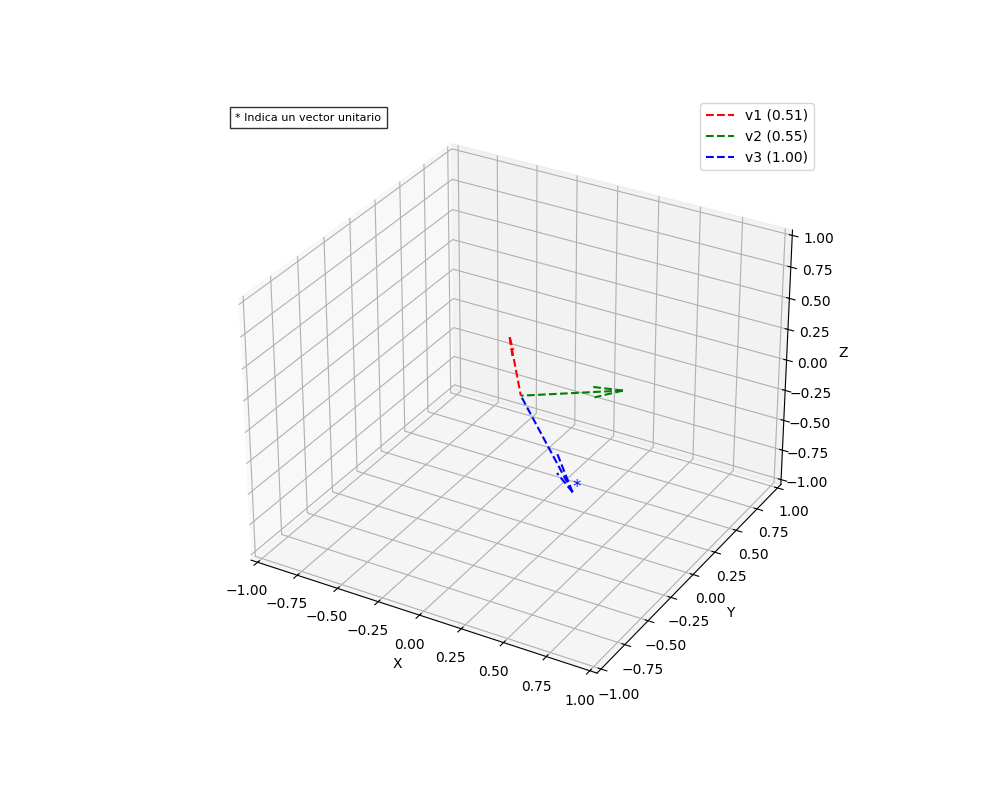
\includegraphics[width=\linewidth]{img/vectors1.png}
    \caption{Representación de los vectores $\mathbf{v_1}$, $\mathbf{v_2}$ y $\mathbf{v_3}$}
    \label{fig:vectors1}
\end{figure}

\textbf{Magnitud del Vector \(\mathbf{v_1}\)}\\

Para \(\mathbf{v_1} = \begin{bmatrix} -0.3 \\ 0.4 \\ 0.1 \end{bmatrix}\):
\[
\|\mathbf{v_1}\| = \sqrt{(-0.3)^2 + 0.4^2 + 0.1^2}
= \sqrt{0.09 + 0.16 + 0.01}
= \sqrt{0.26}
\approx 0.510
\]

\begin{center}
Por lo tanto, no es unitario.\\
\end{center}

\textbf{Magnitud del Vector \(\mathbf{v_2}\)}\\

Para \(\mathbf{v_2} = \begin{bmatrix} 0.5 \\ 0.2 \\ 0.1 \end{bmatrix}\):
\[
\|\mathbf{v_2}\| = \sqrt{0.5^2 + 0.2^2 + 0.1^2}
= \sqrt{0.25 + 0.04 + 0.01}
= \sqrt{0.30}
\approx 0.548
\]

\begin{center}
Por lo tanto, no es unitario.\\
\end{center}

\textbf{Magnitud del Vector \(\mathbf{v_3}\)}\\

Para \(\mathbf{v_3} = \begin{bmatrix} \frac{1}{\sqrt{2}} \\ -\frac{1}{\sqrt{2}} \\ 0 \end{bmatrix}\):
\[
\|\mathbf{v_3}\| = \sqrt{\left(\frac{1}{\sqrt{2}}\right)^2 + \left(-\frac{1}{\sqrt{2}}\right)^2 + 0^2}
= \sqrt{\frac{1}{2} + \frac{1}{2}}
= \sqrt{1}
= 1
\]

\begin{center}
Por lo tanto, es unitario.
\end{center}

\subsection*{2. (15 puntos) Propiedades del producto punto}

Demuestre las siguientes propiedades. Además, muestrelo con una implementación en Pytorch, usando como entrada un arreglo de 50 valores generados al azar, adjunte un pantallazo con la salida de la comparación del resultado a ambos lados de la igualdad, o en su defecto, demuestre el no cumplimiento de la propiedad con un contraejemplo.

\subsubsection*{Supuestos}

Sean \(\mathbf{u} = [u_1, u_2, \dots, u_n]\), \(\mathbf{v} = [v_1, v_2, \dots, v_n]\), y \(\mathbf{w} = [w_1, w_2, \dots, w_n]\) vectores en \(\mathbb{R}^n\), y \(r\) un escalar en \(\mathbb{R}\).

Considere como generalidad que para las demostraciones por código se muestra la inicialización realizada, comprobando la aleatoriedad solicitada:
\begin{lstlisting}[language=Python]
    # Generar vectores aleatorios
    u = torch.rand(50)
    v = torch.rand(50)
    w = torch.rand(50)
    
    # Generar escalar aleatorio
    r = torch.rand(1).item()
\end{lstlisting}

A nivel de los resultados de cada propiedad, se adjuntará el resultado obtenido para cada evaluación.

% -------------------------------------- Propiedad 1 -------------------------------------- %

\subsubsection*{Propiedad 1: Conmutatividad}

\begin{center}
\textbf{Enunciado}: \(\mathbf{u} \cdot \mathbf{v} = \mathbf{v} \cdot \mathbf{u}\)\\
\end{center}

\textbf{Demostración}: El producto punto entre \(\mathbf{u}\) y \(\mathbf{v}\) y \(\mathbf{v}\) y \(\mathbf{u}\) se define respectivamente como:

\[
\mathbf{u} \cdot \mathbf{v} = \sum_{i=1}^{n} u_i v_i
\]

\[
\mathbf{v} \cdot \mathbf{u} = \sum_{i=1}^{n} v_i u_i
\]

Partiendo de la sumatoria derivada de la primera expresión, es posible llegar a la correspondiente sumatoria de la segunda expresión tal como se puede observar a continuación:

\[
\sum_{i=1}^{n} u_i v_i = \sum_{i=1}^{n} v_i u_i
\]

\begin{center}
Por lo tanto, \(\mathbf{u} \cdot \mathbf{v} = \mathbf{v} \cdot \mathbf{u}\)\\
\end{center}

\textbf{Ejercicio demostrativo propuesto:}
\begin{lstlisting}[language=Python]
    dot_uv = torch.dot(u, v)
    dot_vu = torch.dot(v, u)
    
    print(f"u . v = {dot_uv.item()}")
    print(f"v . u = {dot_vu.item()}")
    print(f"Conmutatividad cumple: {torch.isclose(dot_uv, dot_vu)}")
\end{lstlisting}

\textbf{Resultado:}
\begin{lstlisting}
    u . v = 13.014402389526367
    v . u = 13.014402389526367
    Conmutatividad cumple: True
\end{lstlisting}

% -------------------------------------- Propiedad 2 -------------------------------------- %

\subsubsection*{Propiedad 2: Distributividad}

\begin{center}
\textbf{Enunciado}: \(\mathbf{u} \cdot (\mathbf{v} + \mathbf{w}) = \mathbf{u} \cdot \mathbf{v} + \mathbf{u} \cdot \mathbf{w}\)\\
\end{center}

\textbf{Demostración}: Primero, recordemos que el vector correspondiente a \(\mathbf{v} + \mathbf{w}\) también puede expresarse como:

\[
\mathbf{v} + \mathbf{w} = [v_1 + w_1, v_2 + w_2, \dots, v_n + w_n]
\]

Adicionalmente, sabemos que la expresión \(\mathbf{u} \cdot (\mathbf{v} + \mathbf{w})\) también puede presentarse con esta notación:

\[
\mathbf{u} \cdot (\mathbf{v} + \mathbf{w}) = \sum_{i=1}^{n} u_i (v_i + w_i)
\]

Entendiendo que cada componente de los vectores pertenece a \(\mathbb{R}\), se puede reacomodar la sumatoria así, distribuyendo sus componentes internos y separando en dos sumatorias finales:

\[
\sum_{i=1}^{n} u_i (v_i + w_i) = \sum_{i=1}^{n} (u_i v_i + u_i w_i) = \sum_{i=1}^{n} u_i v_i + \sum_{i=1}^{n} u_i w_i
\]

En este punto, es posible regresar a la notación por producto punto donde se obtiene \(\mathbf{u} \cdot \mathbf{v} + \mathbf{u} \cdot \mathbf{w}\).

\begin{center}
Por lo tanto, \(\mathbf{u} \cdot (\mathbf{v} + \mathbf{w}) = \mathbf{u} \cdot \mathbf{v} + \mathbf{u} \cdot \mathbf{w}\)\\
\end{center}

\textbf{Ejercicio demostrativo propuesto:}
\begin{lstlisting}[language=Python]
    dot_u_v_p_w = torch.dot(u, v + w)
    dot_uv = torch.dot(u, v)
    dot_uw = torch.dot(u, w)
    
    print(f"u . (v + w) = {dot_u_v_p_w.item()}")
    print(f"u . v + u . w = {dot_uv.item() + dot_uw.item()}")
    print(f"Distributividad cumple: {torch.isclose(dot_u_v_p_w, dot_uv + dot_uw)}")
\end{lstlisting}

\textbf{Resultado:}
\begin{lstlisting}
    u . (v + w) = 28.568178176879883
    u . v + u . w = 28.56817626953125
    Distributividad cumple: True
\end{lstlisting}

% -------------------------------------- Propiedad 3 -------------------------------------- %

\subsubsection*{Propiedad 3: Multiplicación por escalar}

\begin{center}
\textbf{Enunciado}: \((r \mathbf{u}) \cdot \mathbf{v} = r (\mathbf{u} \cdot \mathbf{v})\)\\
\end{center}

\textbf{Demostración}: Primero, calculamos el vector \(r \mathbf{u}\) similar al primer paso de la propiedad anterior:

\[
r \mathbf{u} = [r u_1, r u_2, \dots, r u_n]
\]

Luego, calculamos el producto punto \((r \mathbf{u}) \cdot \mathbf{v}\) en forma de su sumatoria equivalente:

\[
(r \mathbf{u}) \cdot \mathbf{v} = \sum_{i=1}^{n} (r u_i) v_i
\]

Esta expresión puede desarrollarse aún más extrayendo el escalar \(\mathbf{r}\) de la sumatoria:

\[
\sum_{i=1}^{n} (r u_i) v_i = r \sum_{i=1}^{n} u_i v_i
\]

La sumatoria resultante es equivalente a \(r (\mathbf{u} \cdot \mathbf{v})\).

\begin{center}
Por lo tanto, \((r \mathbf{u}) \cdot \mathbf{v} = r (\mathbf{u} \cdot \mathbf{v})\)\\
\end{center}

\textbf{Ejercicio demostrativo propuesto:}
\begin{lstlisting}[language=Python]
    dot_r_u_v = torch.dot(r * u, v)
    dot_u_v = torch.dot(u, v)
    r_dot_uv = r * dot_u_v
    
    print(f"(r * u) . v = {dot_r_u_v.item()}")
    print(f"r * (u . v) = {r_dot_uv.item()}")
    print(f"Multiplicacion por escalar cumple: {torch.isclose(dot_r_u_v, r_dot_uv)}")
\end{lstlisting}

\textbf{Resultado:}
\begin{lstlisting}
    (r * u) . v = 10.28683853149414
    r * (u . v) = 10.28683853149414
    Multiplicacion por escalar cumple: True
\end{lstlisting}

% -------------------------------------- Propiedad 4 -------------------------------------- %

\subsubsection*{Propiedad 4: Distributividad sobre la suma y escalar}

\begin{center}
\textbf{Enunciado}: \(\mathbf{u} \cdot (r \mathbf{v} + \mathbf{w}) = r (\mathbf{u} \cdot \mathbf{v}) + (\mathbf{u} \cdot \mathbf{w})\)\\
\end{center}

\textbf{Demostración}: Partiendo de lo desarrollado en la \textbf{Propiedad 2} se puede desarrollar la parte izquierda de la siguiente forma:

\[
\sum_{i=1}^{n} u_i (r v_i + w_i) = \sum_{i=1}^{n} (u_i r v_i + u_i w_i) = \sum_{i=1}^{n} u_i r v_i + \sum_{i=1}^{n} u_i w_i
\]

Seguidamente, se aplica \textbf{Propiedad 3} sobre la sumatoria resultante izquierda para reorganizar visualmente la expresión y despejar el escalar:

\[
\sum_{i=1}^{n} u_i (r v_i) = r \sum_{i=1}^{n} u_i v_i
\]

Esto deja la siguiente expresión como resultado general:

\[
\sum_{i=1}^{n} u_i r v_i + \sum_{i=1}^{n} u_i w_i = r \sum_{i=1}^{n} u_i v_i + \sum_{i=1}^{n} u_i w_i
\]

Al regresar a notación vectorial del producto punto obtenemos el resultado final \(r (\mathbf{u} \cdot \mathbf{v}) + (\mathbf{u} \cdot \mathbf{w})\)

\begin{center}
Por lo tanto, \(\mathbf{u} \cdot (r \mathbf{v} + \mathbf{w}) = r (\mathbf{u} \cdot \mathbf{v}) + (\mathbf{u} \cdot \mathbf{w})\)\\
\end{center}

\textbf{Ejercicio demostrativo propuesto:}
\begin{lstlisting}[language=Python]
    dot_u_r_v_p_w = torch.dot(u, r * v + w)
    r_dot_uv = r * torch.dot(u, v)
    dot_u_w = torch.dot(u, w)
    result = r_dot_uv + dot_u_w
    
    print(f"u . (r * v + w) = {dot_u_r_v_p_w.item()}")
    print(f"r * (u . v) + (u . w) = {result.item()}")
    print(f"Distributividad sobre la suma y escalar: {torch.isclose(dot_u_r_v_p_w, result)}")
\end{lstlisting}

\textbf{Resultado:}
\begin{lstlisting}
    u . (r * v + w) = 25.840614318847656
    r * (u . v) + (u . w) = 25.840612411499023
    Distributividad sobre la suma y escalar: True
\end{lstlisting}

% -------------------------------------- Propiedad 5 -------------------------------------- %

\subsubsection*{Propiedad 5: No asociatividad del producto punto}

\begin{center}
\textbf{Enunciado}: \(\mathbf{u} \cdot (\mathbf{v} \cdot \mathbf{w}) \neq (\mathbf{u} \cdot \mathbf{v}) \cdot \mathbf{w}\)\\
\end{center}

\textbf{Demostración por contradicción}: Supongamos que el producto punto es asociativo, es decir:

\[
\mathbf{u} \cdot (\mathbf{v} \cdot \mathbf{w}) = (\mathbf{u} \cdot \mathbf{v}) \cdot \mathbf{w}
\]

Si se desarrollan ambos lados de la igualdad obtenemos individualmente:

\[
\mathbf{u} \cdot (\mathbf{v} \cdot \mathbf{w}) = \mathbf{u} \cdot a
\]

\[
(\mathbf{u} \cdot \mathbf{v}) \cdot \mathbf{w} = b \cdot \mathbf{w}
\]

Con los siguientes valores para cada escalar:

\[
\mathbf{a} = (\mathbf{v} \cdot \mathbf{w}) = \sum_{i=1}^{n} v_i w_i
\]

\[
\mathbf{b} = (\mathbf{u} \cdot \mathbf{v}) = \sum_{i=1}^{n} u_i v_i
\]

Aquí observamos la primera problemática, se está intentado aplicar el operador de producto punto, definido sobre dos vectores, entre un escalar y un vector. \textbf{Contradicción}.\\

\textbf{Ejercicio demostrativo propuesto:}
\begin{lstlisting}[language=Python]
    dot_uv_w = torch.dot(u, torch.dot(v, w))
    dot_u_v_dot_w = torch.dot(torch.dot(u, v), w)
    
    print(f"u . (v . w) = {dot_uv_w.item()}")
    print(f"(u . v) . w = {dot_u_v_dot_w.item()}")
    print(f"Asociatividad cumple: {torch.isclose(dot_uv_w, dot_u_v_dot_w)}")
\end{lstlisting}

\textbf{Resultado:}
\begin{lstlisting}
    RuntimeError                              Traceback (most recent call last)
    Cell In[48], line 2
          1 # Calcular productos punto en distintas formas
    ----> 2 dot_uv_w = torch.dot(u, torch.dot(v, w))
          3 dot_u_v_dot_w = torch.dot(torch.dot(u, v), w)
          5 print(f\"u . (v . w) = {dot_uv_w.item()}\")
    
    RuntimeError: 1D tensors expected, but got 1D and 0D tensors"

    # Se observa un claro error al intentar aplicar operador dot sobre escalar y vector
\end{lstlisting}

De igual forma, si se deseara forzar el uso de la multiplicación, no existe certeza de que el resultado sea igual en ambos lados de la igualdad.

\textbf{Ejercicio demostrativo propuesto:}
\begin{lstlisting}[language=Python]
    dot_uv_w = u * torch.dot(v, w).item()
    dot_u_v_dot_w = torch.dot(u, v).item() * w
    
    print(f"u * (v . w) = {dot_uv_w}")
    print(f"(u . v) * w = {dot_u_v_dot_w}")
    compare_vectors = torch.allclose(dot_uv_w, dot_u_v_dot_w, rtol=1e-5, atol=1e-8)
    print(f"Asociatividad cumple: {compare_vectors}")
\end{lstlisting}

\textbf{Resultado:}
\begin{lstlisting}
u * (v . w) = tensor([ 5.2004,  1.8465,  4.0598,  8.4940,  7.3160,  3.9108,  6.9364,  1.1089,
    7.7678,  8.4213, 12.8140,  9.3583,  5.7158, 11.8077, 11.2251,  9.0907,
    6.3531, 11.2350,  2.3977, 10.8078,  3.9560, 10.0290,  9.1984,  9.7882,
    5.7095,  6.7016,  1.4831,  1.3565,  9.5772,  4.0705,  4.8923,  2.0033,
    8.5814, 10.0672,  9.0177,  3.4351, 11.5927,  0.6206,  1.9212,  4.9786,
   10.0402,  3.1420,  8.3234, 10.7319, 10.2621,  5.2403,  0.5391,  9.2494,
    9.8043, 11.5759])
(u . v) * w = tensor([ 4.3005,  5.5607,  9.1774,  3.7265,  7.7479,  0.7914,  6.6909, 10.4043,
    8.2803,  6.9541,  0.3790,  5.9675,  8.2958, 10.0988,  3.6630,  7.7503,
    4.8988,  9.6043,  6.0584,  8.2298,  3.0009, 12.9015, 11.5620, 12.5870,
    0.2562,  7.0523,  5.3444,  8.6081,  5.5618,  6.4828, 10.6026,  9.7157,
   12.5855, 11.4973, 11.2574,  6.5498, 12.6182, 12.2214,  3.2008, 11.6898,
   12.6560,  3.3989,  3.3404,  3.1903,  0.7170, 12.6289,  8.7186, 11.4072,
   12.4877,  2.6968])
Asociatividad cumple: False
\end{lstlisting}

\begin{center}
Por lo tanto, \(\mathbf{u} \cdot (\mathbf{v} \cdot \mathbf{w}) \neq (\mathbf{u} \cdot \mathbf{v}) \cdot \mathbf{w}\)\\
\end{center}

\section{(40 puntos) Funciones multivariable}
\begin{enumerate}
\item \textbf{(10 puntos)} Funciones lineales multivariable: un hiperplano
definido en un espacio $\mathbb{R}^{n+1}$ se puede expresar como
una función con dominio $\vec{x}\in\mathbb{R}^{n}$ y codominio en
$\mathbb{R}$ como sigue: $z=f\left(\vec{x}\right)=\vec{x}\cdot\vec{w}$,
con $\vec{w}\in\mathbb{R}^{n}$ el arreglo de coeficientes de tal
funcional.
\begin{enumerate}
\item Tómese $\vec{w}_{1}=\begin{bmatrix}0.5\\
0.2
\end{bmatrix}$ para la función $f_{1}$ y $\vec{w}_{2}=\begin{bmatrix}-0.1\\
0.05
\end{bmatrix}$ para la función $f_{2}$, (funciones con dominio en $\mathbb{R}^{2}$
y codominio en ). Grafique ambos planos en Pytorch. 
\item Para cada plano, grafique el vector normal en el punto $P=\left(1,1\right)$
y una curva de nivel perpendicular a tal vector normal. 
\end{enumerate}
\subsection{Respuesta a}

\begin{figure}[H]
    \centering
    \begin{subfigure}[b]{0.45\linewidth}
        \centering
        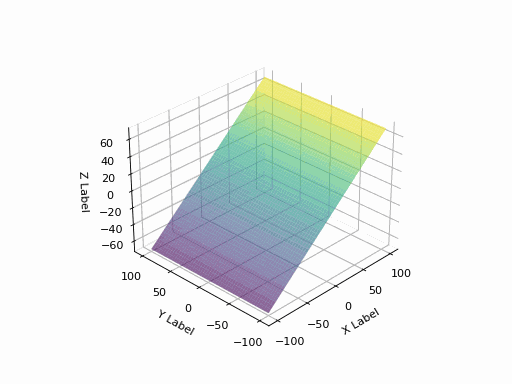
\includegraphics[width=\linewidth]{img/w1.png}
        \caption{Gráfico Hiper plano W1}
        \label{fig:w1}
    \end{subfigure}
    \hfill
    \begin{subfigure}[b]{0.45\linewidth}
        \centering
        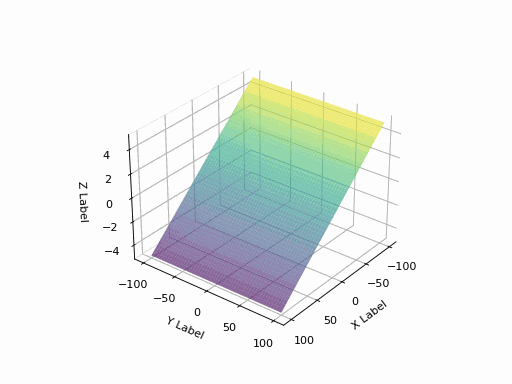
\includegraphics[width=\linewidth]{img/w2.png}
        \caption{Gráfico Hiper plano W2}
        \label{fig:w2}
    \end{subfigure}
    \caption{Gráficos Hiper plano W1 y W2}
    \label{fig:planos}
\end{figure}
\subsection{Respuesta b}
Para graficar el vector normal se convierte la ecuación del plano a su forma cartesiana como se puede observar a continuación:
\[
    ax_1 + bx_2 + \hdots + \alpha x_n + \gamma = 0
\]

Donde los coeficientes son los valores para el vector normal del plano.
\[
    \vec{n} = <a, b, \hdots, \alpha>
\]

Para la primera función el vector normal es el siguiente:
\[
    \vec{n} = <-0.5, -0.2, 1>
\]
 
Para la segunda función el vector normal es el siguiente:
\[
    \vec{n} = <0.1, -0.05, 1>
\]

Para comprobar que esto sea cierto se comprueba que el producto punto del vector normal y cualquier vector que pertenezca al plano debe dar cero. La siguiente función realiza esto para la función 1 y 2 respectivamente.

\begin{lstlisting}
normal = torch.tensor((-0.5, -0.2, 1))
# Punto del plano en 1,1
w1_point = torch.tensor((1,1, 0.7))

print(f"El producto punto es {torch.dot(normal, w1_point)}")
\end{lstlisting}

\begin{lstlisting}
normal = torch.tensor((0.1, -0.05, 1))
# Punto del plano en 1,1
w2_point = torch.tensor((1,1, -0.05))

print(f"El producto punto es {torch.dot(normal, w2_point)}")
\end{lstlisting}

Los siguientes gráficos muestran el vector normal en el plano:
\begin{figure}[H]
    \centering
    \begin{subfigure}[b]{0.45\linewidth}
        \centering
        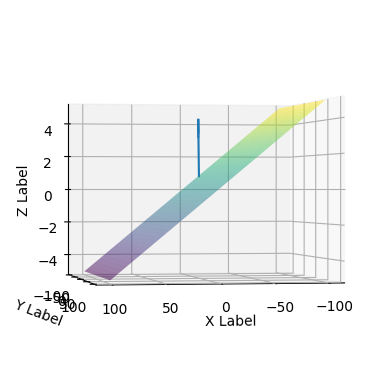
\includegraphics[width=\linewidth]{img/w1_n.png}
        \caption{Gráfico Hiper plano W1}
        \label{fig:w1}
    \end{subfigure}
    \hfill
    \begin{subfigure}[b]{0.45\linewidth}
        \centering
        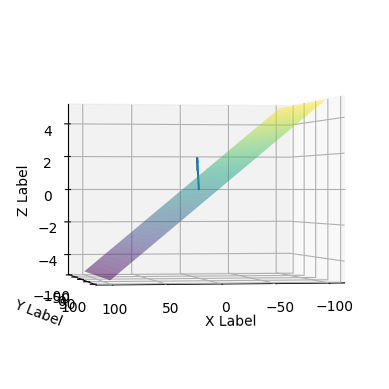
\includegraphics[width=\linewidth]{img/w2_n.png}
        \caption{Gráfico Hiper plano W2}
        \label{fig:w2}
    \end{subfigure}
    \caption{Gráficos Hiper plano W1 y W2 con vector normal}
    \label{fig:planos}
\end{figure}

Para obtener la curva de nivel en el punto P, es necesario saber cual es el valor de $z$ para este punto para obtener el nivel. 

Para la primera función  $z$ se obtiene de la siguiente manera:
\[
    z = (1)*0.5 + (1)*0.2
\]
\[
    z = 0.7
\]
Mientras que para la segunda función es la siguiente:
\[
    z = (1)*-0.1 + (1)*0.05
\]
\[
    z = -0.05
\]

La siguiente figura muestra las curvas de nivel para función 1 y función 2, con z igual a 0.7 y -0.05 respectivamente para las funciones.
\begin{figure}[H]
    \centering
    \begin{subfigure}[b]{0.45\linewidth}
        \centering
        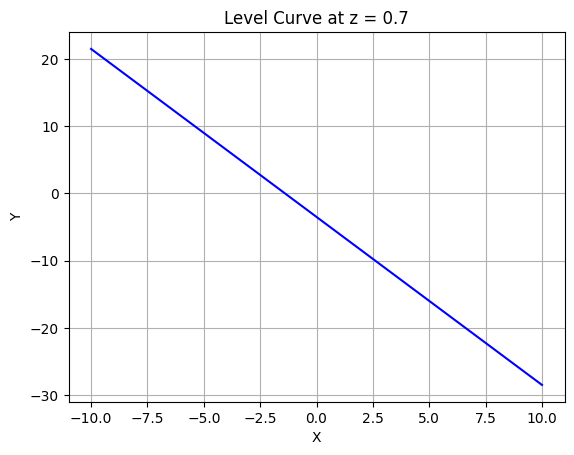
\includegraphics[width=\linewidth]{img/level_w1.png}
        \caption{Curva de nivel w1}
        \label{fig:w1}
    \end{subfigure}
    \hfill
    \begin{subfigure}[b]{0.45\linewidth}
        \centering
        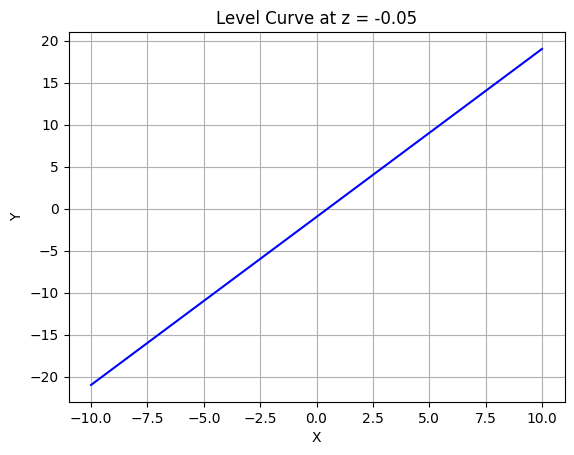
\includegraphics[width=\linewidth]{img/lrvel_w2.png}
        \caption{Curva de nivel w2}
        \label{fig:w2}
    \end{subfigure}
    \caption{Curvas de nivel w1 y w2}
    \label{fig:planos}
\end{figure}


\item \textbf{(30 puntos) El vector gradiente}: Para cada una de las siguientes
funciones multivariable: (1) grafique su superficie con dominio entre
-10 y 10 (2) calcule el vector gradiente manualmente, evaluelo y grafique
el vector unitario en la dirección del gradiente para los dos puntos
especificados (en la misma figura de la superficie) y (3) calcule
la magnitud de tal vector gradiente en cada punto (4) Calcule lo que
se conoce como la matriz Hessiana. 
\begin{enumerate}
\item $f\left(x,y\right)=x^{3}y^{2}+1$, evaluación del gradiente en los
puntos $P_{0}=\left(0,0\right)$ y $P_{1}=\left(7.4,-6.3\right)$.
\item $f\left(x,y\right)=\sin\left(x^{2}\right)+x\cos\left(y^{3}\right)$,
evaluación del gradiente en los puntos $P_{0}=\left(1.5,-5.5\right)$
y $P_{1}=\left(-10,-10\right)$.
\item $f\left(x,y\right)=3^{2x}+5^{4y}+2x+y^{4}$, evaluación del gradiente
en los puntos $P_{0}=\left(-4,-2\right)$ y $P_{1}=\left(-2,9\right)$.
\end{enumerate}
\end{enumerate}
\subsection{Respuesta 1}
Las siguientes figuras muestran los graficos de superficie para las funciones a, b y c.

\begin{figure}[H]
    \centering
    \begin{subfigure}[b]{0.45\linewidth}
        \centering
        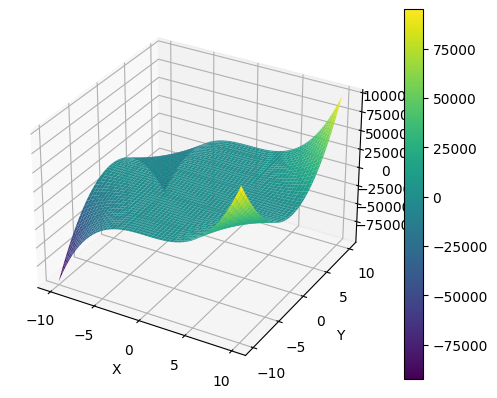
\includegraphics[width=\linewidth]{img/a.png}
        \caption{Gráfico superficie función a}
        \label{fig:w1}
    \end{subfigure}
    \hfill
    \begin{subfigure}[b]{0.45\linewidth}
        \centering
        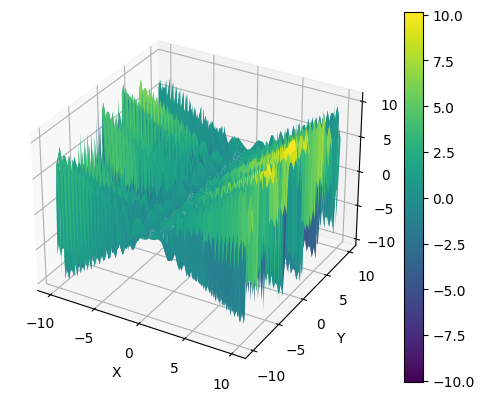
\includegraphics[width=\linewidth]{img/b.png}
        \caption{Gráfico superficie función b}
        \label{fig:w2}
    \end{subfigure}
      \begin{subfigure}[b]{0.45\linewidth}
        \centering
        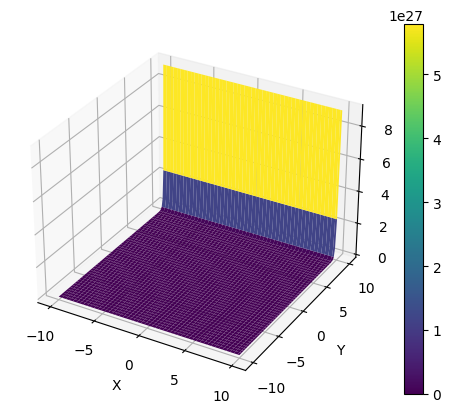
\includegraphics[width=\linewidth]{img/c.png}
        \caption{Gráfico superficie función c}
        \label{fig:w2}
    \end{subfigure}
    \caption{Gráficos Hiper plano W1 y W2 con vector normal}
    \label{fig:planos}
\end{figure}
\subsection{Respuesta 2}
Para calcular el vector gradiente se emplea la siguiente función, donde cada elemento es una derivada parcial de $f$ en con respecto a las dimensiones.
\[
\nabla f(p) = \begin{bmatrix}
 \frac{\partial f}{\partial x_1}(p) \\
 \vdots \\
 \frac{\partial f}{\partial x_n}(p)
\end{bmatrix}
\]

\subsubsection{Función a}
Para obtener el vector gradiente es necesario obtener las derivadas parciales con respecto a $x$ y $y$. A continuación se muestran estas derivadas:
\[
    f_x = 3x^2y^2
\]
\[
    f_y = 2x^3y
\]

Estas forman el vector gradiente de $f$
\[
    \nabla f = ( \frac{\partial f}{\partial x},  \frac{\partial f}{\partial y})
\]

\[
    \nabla f = ( 3x^2y^2,  2x^3y)
\]

En los puntos $P_0$ y $P_1$ el vector tiene los siguientes valores:
\[
    \nabla f(P_0) = ( 3(0)^2(0)^2,  2(0)^3(0))
\]

\[
    \nabla f(P_0) = ( 0,  0)
\]

\[
    \nabla f(P_1) = ( 3(7.4)^2(-6.3)^2,  2(7.4)^3(-6.3))
\]

\[
    \nabla f(P_1) = ( 6520.2732,  -5105.8224)
\]

Al colocar el graficar el vector en los puntos se tiene la siguiente imagen.
\begin{figure}[H]
    \centering
    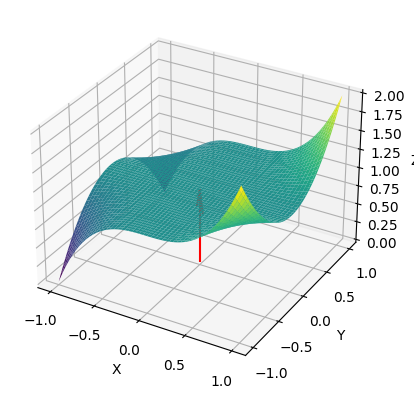
\includegraphics[width=0.5\linewidth]{img/a_v.png}
    \caption{Función con el vector gradiente de $P_0$ a $P_1$}
    \label{fig:enter-label}
\end{figure}

\subsubsection{Función b}
Para obtener el vector gradiente es necesario obtener las derivadas parciales con respecto a $x$ y $y$. A continuación se muestran estas derivadas:
\[
    f_x = 2xcos(x^2) - sin(y^3)
\]
\[
    f_y = -3xy^2cos(y^3)
\]

Estas forman el vector gradiente de $f$
\[
    \nabla f = ( \frac{\partial f}{\partial x},  \frac{\partial f}{\partial y})
\]

\[
    \nabla f = ( 2xcos(x^2) - sin(y^3),  -3xy^2cos(y^3))
\]

En los puntos $P_0$ y $P_1$ el vector tiene los siguientes valores:
\[
    \nabla f(P_0) = (  2(1.5)cos((1.5)^2) - sin((-5.5)^3),  -3(1.5)(-5.5)^2cos((-5.5)^3))
\]

\[
    \nabla f(P_0) = ( -1.755471,  134.9867394)
\]

\[
    \nabla f(P_1) = ( 3(7.4)^2(-6.3)^2,  2(7.4)^3(-6.3))
\]

\[
    \nabla f(P_1) = ( -16.41949,  1687.137228)
\]

Al colocar el graficar el vector en los puntos se tiene la siguiente imagen.
\begin{figure}[H]
    \centering
    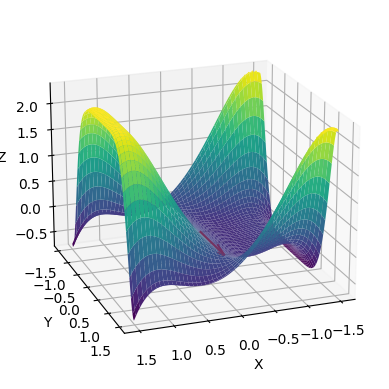
\includegraphics[width=0.5\linewidth]{img/b_v.png}
    \caption{Función con el vector gradiente de $P_0$ a $P_1$}
    \label{fig:enter-label}
\end{figure}

\subsubsection{Función c}
Para obtener el vector gradiente es necesario obtener las derivadas parciales con respecto a $x$ y $y$. A continuación se muestran estas derivadas:
\[
    f_x = 2\ln \left(3\right) \:9^x+2
\]
\[
    f_y = 4y^3+4\ln \left(5\right) \:625^y
\]

Estas forman el vector gradiente de $f$
\[
    \nabla f = ( \frac{\partial f}{\partial x},  \frac{\partial f}{\partial y})
\]

\[
    \nabla f = ( 2\ln \left(3\right) \:9^x+2,  4y^3+4\ln \left(5\right) \:625^y)
\]

En los puntos $P_0$ y $P_1$ el vector tiene los siguientes valores:
\[
    \nabla f(P_0) = ( 2\ln \left(3\right) \:9^(-4)+2, 4(-2)^3+4\ln \left(5\right) \:625^(-2))
\]

\[
    \nabla f(P_0) = ( 2.0003, -31.9999)
\]

\[
    \nabla f(P_1) = ( 2\ln \left(3\right) \:9^(-2)+2, 4(9)^3+4\ln \left(5\right) \:625^(9))
\]

\[
    \nabla f(P_1) = ( 2.0271,  9.3681)
\]

Al colocar el graficar el vector en los puntos se tiene la siguiente imagen.
\begin{figure}[H]
    \centering
    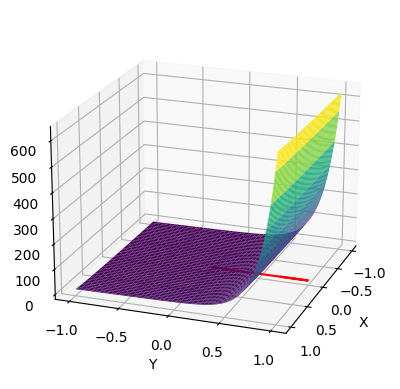
\includegraphics[width=0.5\linewidth]{img/c_v.png}
    \caption{Función con el vector gradiente de $P_0$ a $P_1$}
    \label{fig:enter-label}
\end{figure}
\subsection{Respuesta 3}
Para calcular la magnitud del vector gradiente en los puntos se utiliza la norma euclidiana:
\[
\mathbf{x}\| = \sqrt{x_1^2 + x_2^2 + \cdots + x_n^2}
\]
\subsubsection{Función a}
Para calcular la magnitud de los vectores gradientes, se necesita el valor en el eje Z, para esto se evalúa el vector gradiente en la función original.


\[
\|\mathbf{P_0}\| = \sqrt{0^2 +  0^2}
\]

\[
\|\mathbf{P_1}\| = \sqrt{6520.2732^2 +  -5105.8224^2}
\]

\[
\|\mathbf{P_0}\| = 0
\]

\[
\|\mathbf{P_1}\| = 8281.5
\]

\subsubsection{Función b}
Para calcular la magnitud de los vectores gradientes, se necesita el valor en el eje Z, para esto se evalúa el vector gradiente en la función original.


\[
\|\mathbf{P_0}\| = \sqrt{-1.755471^2 +  134.9867394^2}
\]

\[
\|\mathbf{P_1}\| = \sqrt{-16.41949^2 +  1687.137228^2}
\]

\[
\|\mathbf{P_0}\| = 134.99
\]

\[
\|\mathbf{P_1}\| = 1687.21
\]

\subsubsection{Función c}
Para calcular la magnitud de los vectores gradientes, se necesita el valor en el eje Z, para esto se evalúa el vector gradiente en la función original.


\[
\|\mathbf{P_0}\| = \sqrt{2.0003^2 + -31.9999^2}
\]

\[
\|\mathbf{P_1}\| = \sqrt{2.0271^2 + 9.3681^2}
\]

\[
\|\mathbf{P_0}\| = 32.06235
\]

\[
\|\mathbf{P_1}\| = 9.5849
\]


\subsection{Respuesta 4}
Para calcular la matriz hessiana se emplea la siguiente formula:
\[
\mathbf H_f= \begin{bmatrix}
  \dfrac{\partial^2 f}{\partial x_1^2} & \dfrac{\partial^2 f}{\partial x_1\,\partial x_2} & \cdots & \dfrac{\partial^2 f}{\partial x_1\,\partial x_n} \\[2.2ex]
  \dfrac{\partial^2 f}{\partial x_2\,\partial x_1} & \dfrac{\partial^2 f}{\partial x_2^2} & \cdots & \dfrac{\partial^2 f}{\partial x_2\,\partial x_n} \\[2.2ex]
  \vdots & \vdots & \ddots & \vdots \\[2.2ex]
  \dfrac{\partial^2 f}{\partial x_n\,\partial x_1} & \dfrac{\partial^2 f}{\partial x_n\,\partial x_2} & \cdots & \dfrac{\partial^2 f}{\partial x_n^2}
\end{bmatrix}
\]

\subsubsection{Funcion a}
Primera se calcula la primera derivada parcial con respecto a "x" y "y".
\[
    f_x = 3x^2y^2
\]
\[
    f_y = 2x^3y
\]

Después se calcula la matriz empleando estas derivadas:
\[
f_{xx} = 6 x y^2
\]
\[
f_{xy} = 6 x^2 y
\]
\[
f_{yx} = 6 x^2 y
\]
\[
f_{yy} =  2 x^3
\]

Con estas derivadas se obtiene la siguente matriz hessiana:
\[
\mathbf H_{fa}= \begin{bmatrix}
  f_{xx} & f_{xy} \\
  f_{yx} & f_{yy}
\end{bmatrix}
\]

\[
\mathbf H_{fa}= \begin{bmatrix}
  6 x y^2 & 6 x^2 y \\
  6 x^2 y & 2 x^3
\end{bmatrix}
\]

\subsubsection{Función b}
Primera se calcula la primera derivada parcial con respecto a "x" y "y".
\[
    f_x = 2xcos(x^2) - sin(y^3)
\]
\[
    f_y = -3xy^2cos(y^3)
\]

Después se calcula la matriz empleando estas derivadas:
\[
f_{xx} = 2 cos(x^2) - 4 x^2 sin(x^2) 
\]
\[
f_{xy} = -3 y^2 sin(y^3)
\]
\[
f_{yx} = -3 y^2 sin(y^3)
\]
\[
f_{yy} =  -6 x y sin(y^3) - 9 x y^4 cos(y^3)
\]

Con estas derivadas se obtiene la siguente matriz hessiana:
\[
\mathbf H_{fb}= \begin{bmatrix}
  f_{xx} & f_{xy} \\
  f_{yx} & f_{yy}
\end{bmatrix}
\]

\[
\mathbf H_{fa}= \begin{bmatrix}
  2 cos(x^2) - 4 x^2 sin(x^2)  & -3 y^2 sin(y^3) \\
  -3 y^2 sin(y^3) & -6 x y sin(y^3) - 9 x y^4 cos(y^3)
\end{bmatrix}
\]

\subsubsection{Función c}
Primera se calcula la primera derivada parcial con respecto a "x" y "y".
\[
    f_x = 2\ln \left(3\right) \:9^x+2
\]
\[
    f_y = 4y^3+4\ln \left(5\right) \:625^y
\]

Después se calcula la matriz empleando estas derivadas:
\[
f_{xx} = 4 3^(2 x) log^2(3)
\]
\[
f_{xy} = 0
\]
\[
f_{yx} = 0
\]
\[
f_{yy} =  12 y^2 + 16 5^(4 y) log^2(5)
\]

Con estas derivadas se obtiene la siguente matriz hessiana:
\[
\mathbf H_{fb}= \begin{bmatrix}
  f_{xx} & f_{xy} \\
  f_{yx} & f_{yy}
\end{bmatrix}
\]

\[
\mathbf H_{fa}= \begin{bmatrix}
 4 \cdot 3^{(2x)} log^2(3)  & 0 \\
  0 & 12 y^2 + 16\cdot5^{(4 y)} log^2(5)
\end{bmatrix}
\]
\end{document}